\section*{Explicaci\'on de la Arquitectura}


\subsection*{Diagrama de Componentes y Conectores}

\subsubsection*{Visi\'on global de la arquitectura}

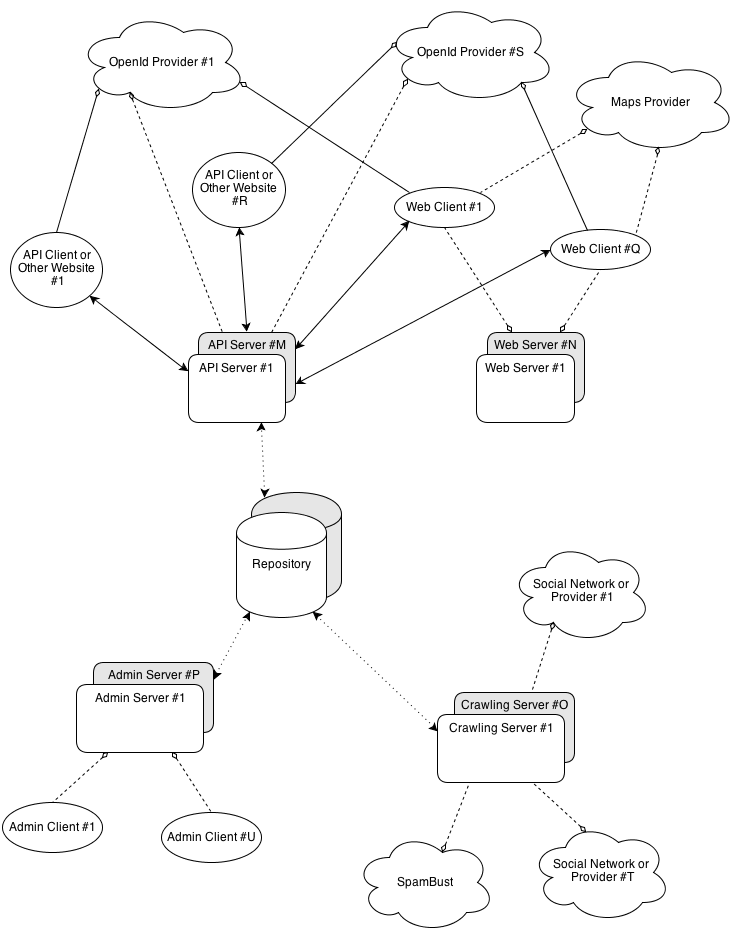
\includegraphics[scale=0.5]{ISW2_cNc_Global}


\subsubsection*{Consulta Web o API}

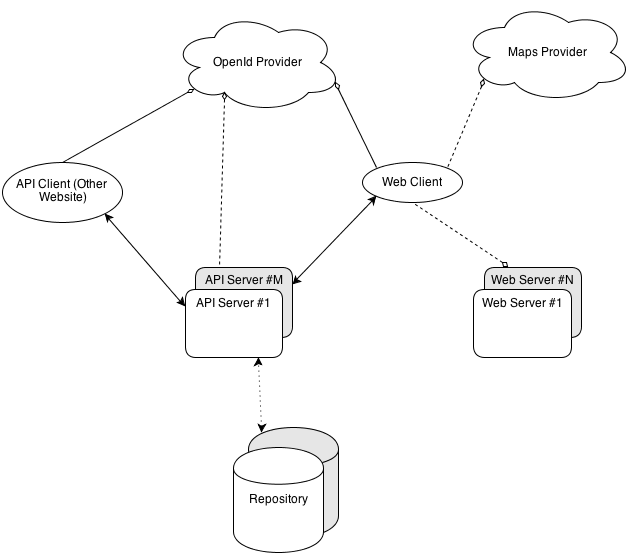
\includegraphics[scale=0.5]{ISW2_cNc_Consulta}

En el diagrama de la consulta web se identifican dos tipos de clientes, que son los clientes del sitio Web y los que consumen \'unicamente la API web. Tenemos tambi\'en dos tipos de componenetes servidor propios, que son los servidores del sitio Web y el servidores de la API web. Adem\'as, el diagrama nos muestra el repositorio de datos de configuraci\'on y consulta. Por \'ultimo, tenemos distintos tipos de servicios externos que son consumidos por los componentes anteriores, como son los proveedores de OpenId y el proveedor de mapas.

Los clientes Web consumen el contenido est\'atico directamente de los servidores del sitio Web, como puede ser el contenido HTML, JS, CSS e im\'agenes; se puede ver que el conector es de tipo cliente/servidor, lo que representa la sesi\'on que arma el navegador con el servidor, y el bloqueo del thread de UI principal entre sucesivos requests (GET principalmente). En principio, este tipo de interacci\'on es lo m\'as simple posible, sin nig\'un tipo de autenticaci\'on; la mayor parte del contenido es cacheable y compone la UI de la aplicaci\'on (no tiene datos sensibles).

Tanto los clientes Web como los clientes de la API (como pueden ser otros sitios web) interact\'uan con el componente servidor API.

La autenticaci\'on es resuelta como parte de esta interacci\'on, de acuerdo a la especificaci\'on de OpenId (\url{http://openid.net/specs/openid-authentication-2_0.html}):

\begin{itemize}
\item el cliente informa al componente servidor API el proveedor de OpenId que va a utilizar
\item el componente API establece una sesi\'on con el proveedor elgido (representamos esta sesi\'on con un conector de tipo cliente/servidor) que podr\'a ser reutilizada para subsiguientes validaciones o para obtener datos extra del mismo cliente
\item el cliente es redireccionado con el proveedor elegido para realizar la autenticaci\'on (representamos esta interacci\'on como un env\'io de un mensaje a trav\'es de una conexi\'on sincr\'onica)
\item el componente API reutiliza la sesi\'on establecida con el proveedor para verificar la informaci\'on de autenticaci\'on y para obtener datos adicionales
\end{itemize}

M\'as all\'a de manejar la autenticaci\'on, el componente servidor API responde a todos los pedidos de b\'usqueda o datos de configuraci\'on, de manera indistinta entre clientes Web o de API (usar\'ian el mismo puerto); el tipo de conexi\'on en este caso es asincr\'onica en ambos sentidos, para representar llamados tipo AJAX.

La interacci\'on con el proveedor de mapas asumimos que se puede resolver directamente desde el cliente, mediante alg\'un tipo de plugin descargado est\'aticamente desde el sitio Web.

El acceso al repositorio de datos y configuraci\'on lo hace \'unicamente el componente servidor API, para poder satisfacer los distintos requests, que agrupar\'ian todo el contenido din\'amico de la aplicaci\'on.

Por \'ultimo vale destacar que la cardinalidad del componente servidor API puede ser distinta a la del componente servidor Web, y dado que el primero atiende a consultas din\'amicas, con workflows m\'as complejos (como el de autenticaci\'on), y con mayor utilizaci\'on de recursos, podr\'ia ser necesario escalarlo en mayor medida que al segundo, que s\'olo responde a requests de contenido est\'atico. Adem\'as s\'olo es necesario implementar el proceso de autenticaci\'on en el componente servidor API, sustentado por el hecho de que s\'olo \'este tiene acceso al repositorio, simplificando la arquitectura.


\subsection*{Diagrama de Alocaci\'on}


\subsection*{Arquitectura y Calidad}

